\documentclass[12pt]{article}
\usepackage[legalpaper,margin=.6in]{geometry}
\usepackage{graphicx}
\usepackage{amsmath}
\usepackage{fontspec}
\setmainfont{Amerigo BT}
\usepackage{float}
\usepackage{tabto}
\usepackage{caption}
\usepackage{setspace}
\usepackage{hyperref}
\hypersetup{
    colorlinks,
    citecolor=black,
    filecolor=black,
    linkcolor=black,
    urlcolor=black
}
\newcommand\myeq{\mathrel{\stackrel{\makebox[0pt]{\mbox{\normalfont\tiny def}}}{=}}}

\setlength{\parindent}{0em}
\setlength{\fboxsep}{0em}
\setlength{\fboxrule}{1pt}
\begin{document}
{\setmainfont{Times New Roman}
\begin{center}
    
    \topskip0pt
    \vspace*{\fill}
    \textbf{\huge Probabilistic Fracture Simulation}
   \textbf{\\[.75in]\Large A SEMINAR REPORT\\~\\}
    \textit{\large Submitted in the partial fulfillment of the award of the degree of}\\[.55in]
    \textbf{\Large MASTER OF TECHNOLOGY}\\~\\\textit{\Large in}\\~\\ \textbf{\Large STRUCTURAL ENGINEERING}
    \\~\\~\\~\\{\Large By}\\~\\  \textbf{\Large ABHINANDAN SHARMA}\\~\\~\\
    Under the Guidance of
    \textbf{\\~\\\Large PROF. RAJIB CHOWDHURY}\\~\\~\\
    
\includegraphics[width=.3\textwidth]{iitr.png}\\~\\~\\
    {\bf\large STRUCTURAL ENGINEERING GROUP\\~\\
DEPARTMENT OF CIVIL ENGINEERING\\~\\
INDIAN INSTITUTE OF TECHNOLOGY ROORKEE\\~\\
ROORKEE- 247667, UTTARAKHAND, INDIA.\\~\\
MAY 2021}
    \vspace*{\fill}
\end{center}
\pagebreak  

%----------------------------------------------------------------
\begin{center}
\textbf{ \LARGE   INDIAN INSTITUTE OF TECHNOLOGY ROORKEE\\
ROORKEE - 247667\\~\\

\includegraphics[width=.3\textwidth]{iitr.png}\\~\\
\underline{CANDIDATE'S DECLARATION}\\}
\end{center}
\begin{doublespace}
    {\large I hereby declare that work being presented in this report, entitled \textbf{\large "Probabilistic Fracture Simulation"} 
    towards partial fulfillment of the requirements for the award of the degree of \textbf{\large "Master of Technology in Structural Engineering"}
    submitted to
    the Department of Civil Engineering, Indian Institute of Technology, Roorkee, is an authentic
    record of my own work carried out under the guidance of \textbf{Dr. Rajib Chowdhury}, Associate
    Professor, Department of Civil Engineering, IIT Roorkee.\\~\\
    The matter presented in this thesis has not been submitted by me for the award of any other
    degree of this or any other Institute. \\~\\
    }    
\end{doublespace}
\begin{minipage}[t]{7cm}\bf
\flushleft
Date:\\Place:\\
\end{minipage}
\hfill
\begin{minipage}[t]{7cm}\bf
\flushright
(ABHINANDAN SHARMA)\\
\end{minipage}
\\~\\
\begin{center}\bf
    \LARGE \underline{COUNTERSIGNED}\\
\end{center}
This is to certify that the above statement made by the candidate is correct to the best of my
knowledge.\\~\\
\begin{minipage}[t]{5cm}\bf
    \flushleft
    Date:\\Place:\\
    \end{minipage}
    \hfill
    \begin{minipage}[t]{10cm}\bf
    \flushright
    Dr. Rajib Chowdhury
\\Associate Professor,
\\Department of Civil Engineering,
\\Indian Institute of Technology,
\\Roorkee
\\Roorkee – 247667 (INDIA)\\
    \end{minipage}

\pagebreak
\begin{center}
    \textbf{ \LARGE   INDIAN INSTITUTE OF TECHNOLOGY ROORKEE\\
    ROORKEE - 247667\\~\\
    
\includegraphics[width=.3\textwidth]{iitr.png}\\~\\
    \underline{ACKNOWLEDGEMENT}\\}
    \end{center}
    \begin{doublespace}
        {\large I would like to thank and express my deepest sense of gratitude and indebtedness to my Ph.D.
        supervisor \textbf{Dr. Rajib Chowdhury}, Associate Professor, Department of Civil Engineering, IIT
        Roorkee, for his valuable guidance, encouragement and generous assistance throughout in
        putting together this seminar report. This work is simply the reflection of his thoughts, ideas,
        concepts and all his efforts. I am highly indebted to him for his kind and valuable suggestions
        and of course his valuable time during the period of the work.\\
        I would acknowledge my gratefulness to my seniors and friends who provided valuable
        suggestions and encouragement whenever I needed. I am also extremely grateful to my family
        members for their support, love, patience and for being a constant source of inspiration.\\~\\
        }    
    \end{doublespace}

    \begin{minipage}[t]{7cm}\bf
        \flushleft

        Date:\\
        \end{minipage}
        \hfill
        \begin{minipage}[t]{7cm}\bf
        \flushright
            ABHINANDAN SHARMA
        \end{minipage}

\pagebreak
%------------------------------------------------------------------
}
\tableofcontents
\pagebreak
\listoffigures
\pagebreak
\rule{\textwidth}{.1em}
\begin{center}
\textbf{Abstract}
\end{center}
This seminar topic focuses on the Fundamentals of the fracture mechanics based on the crack tip stress and strain fields and the non-linear fracture mechanics have been developed. Their applications to the studies of fracture initiation and stable crack growth may differ because of the difference in the basic postulates of various fracture theories.
    the impact of computational methodology on furthering the understanding of fundamental fracture phenomena. The current numerical approaches to the solution of fracture mechanics problems.
    the methodology for probabilistic fracture mechanics analysis (PFM) of structural components with crack-like imperfections. Details are given for the development and application of both a simple nomographic method and a basic numerical tool for PFM applications.

    

\rule{\textwidth}{.1em}

%------------------------------------------------------------------
%------------------------------------------------------------------

\section{Fundamental Basis Of Fracture Mechanics}
Inglis made the stress analysis of an elliptical hole in a uniformly stressed elastic plate. A crack can be 
represented by an infinitesimally narrow ellipse. Based on Inglis elastic stress solution to a cracked solid. 
Griffith formulated his well known energy criterion for brittle fractures. At the fracture initiation of a cracked brittle solid in the 
condition of fixed grip, the release rate of the stored strain energy equals or exceeds the dissipative surface energy rate.
\(\partial U_\epsilon / \partial a \geq \partial U_s / \partial a = 2 \gamma \), 
where $U_\epsilon$ and $U_S$ are strain energy and surface energy; $\gamma$,  the surface energy per unit area; and $a$, crack length.$\gamma$ 
is constant for a given material. Assuming a constant dissipative rate of plastic energy $\varGamma $ , 
Irwin and Orowan extended the energy criterion to metallic solids, where plastic deformation takes place at crack tips.
\\\\The crack tip elastic stresses, strains and displacements are characterized by the stress intensity factor, $K$.  
Incase of small scale yielding, $SSY, K$ characterizes crack tip stresses, strains, and displacements even within a 
crack tip plastic zone in a metallic specimen. $K$ characterizes cracktip
stresses, strains and displacements forms the fundamental basis of the linear elastic fracture mechanics rather than 
the global energy balance. More recently, Hutchinson, and Rice and Rosengren derived the crack tip stress, strain and 
displacement fields in power law strain hardening 
materials. The crack tip stress, strain and displacement 
fields can be characterized by $J$, which is a contour independent 
integral. $J$ is also the rate of potential energy change during 
the cracking process in a non-linear elastic solid. $J$ has been 
widely used to study non-linear fracture mechanics.
\subsection{Defining Fracture}Figure shows a cracked sample and its load P vs load point displacement, $\delta$. The “crack” suddenly starts to propagate internally at A. The increased crack length increases the compliance of the specimen and causes the sudden load drop from A to A'. As the load increases, the crack continues its internal growth. At B, the crack front at the specimen surface starts to move forward, and the crack continues to grow in a “stable” manner to the maximum load C. D is the point of final separation, fracture mechanics studies the fracture initiation at A and the stable crack growth from A' to B and onwards. Often the point of fracture initiation is not so clearly defined as shown in the figure. In this case, certain degree of arbitrariness has to be introduced in order to define fracture initiation. Fracture can be defined in terms of the above described macro-features or in terms of the micro-structural features such as fracture of brittle inclusions,etc.
\begin{figure}[H]
    \centering
    \fbox{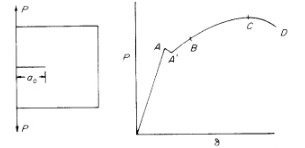
\includegraphics[width=.5\textwidth]{s1.png}}
    \captionsetup{labelformat=empty}
    \caption{load-elongation curve for fracture initiation and stable crack growth}  
\end{figure}
\subsection{Elastic Stress Field}Linear elastic fracture mechanics (LEFM) is based on the elastic solution of the crack tip stress field. Williams has shown that in a cracked plate 
$\sigma_{ij}$, $\epsilon_{ij}$ and $u_i$ can be expressed in terms of:

\begin{align*}
    \sigma_{ij}(r, \theta) &= \frac{k_1}{\sqrt{2 \pi r}} \bar{\sigma}_{ij(1)}(\theta) + k_2 \bar{\sigma}_{ij(2)}(\theta) + k_3 \sqrt{(2 \pi r)}\bar{\sigma}_{ij(3)}(\theta) + ...
    \\\epsilon_{ij}(r, \theta) &= \frac{k_1}{\sqrt{2 \pi r}} \bar{\epsilon}_{ij(1)}(\theta) + ... \tag{1} \label{1}
    \\u_{ij}(r, \theta) &= \frac{k_1 \sqrt{(2 r)}}{\pi} \bar{u}_{i(1)}(\theta) + ...
\end{align*}


where $r$ and $\theta$ are polar coordinates, the crack tip is located at the origin of the reference system, and
the crack line coincides with the line $\theta = \pi, \bar{\sigma}_{ij}, \bar{\epsilon}_{ij}$ and $, \bar{u}_{i}$ give the distributions of their corresponding 
stress, strain, and displacement components. $k_1, k_2, k_3. . .$ are 
prescribed by specimen geometry and boundary conditions.
Fracture takes place at the crack tie: therefore, we have 
to consider only the stresses and strains in the immediate 
vicinity of a crack tip. In this region, the first singular terms of 
these series dominate the stress and strain fields. Irwin writes these singular 
terms for mode I tensile cracks in the following form:
\begin{align*} 
    \sigma_{ij}(r, \theta) &= \frac{K_I}{\sqrt{2 \pi r}} \bar{\sigma}_{ij}(\theta) 
    \\\epsilon_{ij}(r, \theta) &= \frac{K_I}{\sqrt{2 \pi r}} \bar{\epsilon}_{ij}(\theta) \tag{2} \label{2}
    \\u_{ij}(r, \theta) &= \frac{K_I \sqrt{(2 r)}}{\pi} \bar{u}_{i}(\theta)
\end{align*}
\\The elastic stress or strain field can be separated into two parts dealing with stress distribution and is a function of the coordinates alone.
 In cracked solids this is $\bar{\sigma}_{ij}(\theta)/\sqrt{(2 \pi r)}$ and 
 the other part is $K$, or the "stress intensity factor".
If $K_I$ is known, all $\bar{\sigma}_{ij}, \bar{\epsilon}_{ij}$ and $, \bar{u}_{i}$ are known. Therefore, 
$K_I$ characterizes crack tip stresses, strains, and displacements.
Equatione \eqref{2} approximates characteristic creack tip elastic field zone, $r_e$
\\\\As a crack propagates, the stored strain energy in the plate changes. The strain energy change can be
calculated. Figure shows the contour of a crack tip under stress. Apply stress $\sigma_{yy}$ in the crack
increment $\Delta a$. As $\sigma_{yy}$ increases, the two mating crack surfaces close. The necessary work done to close
the crack within $\Delta a$ is:
\begin{align*}
    \Delta W = \int_{0}^{\Delta a} \sigma_{yy}(r', 0)u_y(r, \pi)dr = \frac{(1 - \nu ^ 2)}{E} K_{I}^2 \Delta a \tag{3} \label{3}
\end{align*}
\begin{figure}[H]
    \centering
    \fbox{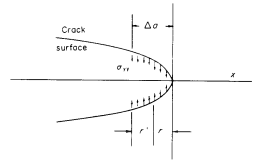
\includegraphics[width=.4\textwidth]{s3.png}}
    \captionsetup{labelformat=empty}
    \caption{word done to close the crack increment $\Delta a$}
    
\end{figure}


for the plane strain case. This is also the amount of strain energy released as the crack moves forward
under the fixed grip condition. It can be considered as the strain energy flux which flows toward the
crack tip during fracturing.
\\\\The rate of the strain energy flux is denoted by G and is also known as crack extension force.
\begin{align*}
    G_I = K_{I}^{2}/\bar{E} \tag{4} \label{4}
\end{align*}
where $\bar E = E/(1 - \nu^2)$ for plain strain case and $\bar{E} = E$ for plane stress.






\subsection{Griffith Criterion}
Griffith proposed the criterion of brittle fracture based on the principle of global energy balance.
\begin{align}
    \frac{\partial}{\partial a}(U_\epsilon + U_\gamma) = 0 \tag{5} \label{5}
\end{align}
where $U_\epsilon$  is the strain energy and $U_\gamma$ is the surface energy.
\begin{align*}
    &G = -\frac{\partial U_\epsilon}{\partial a} \\ &and \\ &\frac{\partial U_\gamma}{\partial a} = 2 \gamma
\end{align*}
which is constant. For a small crack in a large plate, we habbve, at fracture.
\begin{align*}
    &G_c = (1 - \nu ^ 2)\frac{\sigma_{c} ^ 2 \pi a}{E} = 2 \gamma \\ &and \\ &\sigma_c = \sqrt{\frac{2 \gamma E}{(1 - \nu ^ 2)\pi a } }
    \\\\\text{Hence, \ \ \ \ \ \ \ \ \ \ \ \ \ } & \sigma_c \sqrt{(\pi a)} = \text{material constant}
\end{align*}
Hence, for perfectly brittle solid $k$ characterizes $\sigma_{ij}$ and $\epsilon_{ij}$.
For same material and same crack tip elastic stresses and strains, the $K_c$(critical value) must be constant.
\begin{align*}
    K_c = \sigma_c \sqrt{(\pi a)} = \text {constant}
\end{align*}

\subsection{The Extension Of The Griffith Criterion}
A correct fracture theory should agree with know fracture phenomena. If not, the analysis must 
be wrong. The fracture stress, $\sigma_c$, of a large specimen with a long crack is lower
than the fracture stress of a small specimen with a short crack as shown schematically in figure
below.


\begin{figure}[H]
    \centering
    \fbox{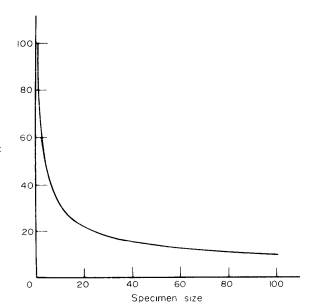
\includegraphics[width=.4\textwidth]{s4.png}}
    \captionsetup{labelformat=empty}
    \caption{Fracture stress of geometrically similar specimens, same thcikness, same material}
\end{figure}

\subsubsection{Global Energy Balance Theory}
At fracture we have:
\begin{align*}
    \frac{\partial}{\partial a}(U_\gamma + U_\epsilon + U_p) = 0 \tag{6} \label{6}
\end{align*}

$U_\gamma$ is surface energy; $U_\epsilon$ is strain energy; and $U_p$ is plastic work. 
It is known that $U_\gamma \ll U_p$. Neglect $U_\gamma$, we get: 
\begin{align*}
    \frac{\partial}{\partial a}(U_\epsilon + U_p) = 0 \tag{7} \label{7}
\end{align*}

This leads to $G_c = (\partial U_p/\partial a)$. In infinite metallic
plate in the condition that strain prevails due to enough thickness. As
cracks extend under $\sigma_\infty$, the relation between work dissipation $U_p$
and crack lengh "2$a$" can be found. The classic plasticity theory shows, $r_p \propto a$ ,
and $U_p \propto r_{p} ^{2}$ which gives

\begin{align*}
    \frac{\partial U_p}{\partial a} = Ca
\end{align*}
C is proportionality constant, which gives:
\begin{align}
    \frac{\sigma_{c}^{2} \pi a (1 - \nu ^ 2)}{E} = Ca \qquad
\Rightarrow \qquad &\sigma_c = \sqrt{\frac{CE}{\pi (1 - \nu ^ 2)}} = \text{constant} \nonumber
\end{align}

The experimental evidences that demonstrate the failure of the global energy balance are well known.
But they have not been recognized as such. Figure shows the thickness effects on fracture toughness.
The fracture toughness varies from 40 MPa$\sqrt{\text{m}}$ for $K_{Ic}$, to the maximum value of 107 MPa$\sqrt{\text{m}}$. The
strain energy release rates of the two limiting cases of plane strain and plane stress states differ by a
factor of $(1 - \nu ^ 2)$. $v$ is Poisson’s ratio. The difference is approximately 10\%. If the plastic energy
dissipation rate is constant, the difference in fracture toughnesses should not be more than 10\%. The
large difference in the observed fracture toughnesses in Figure, from the point of view of energy balance,
must arise from the difference in plastic energy dissipation rates.

\begin{figure}[H]
    \centering
    \fbox{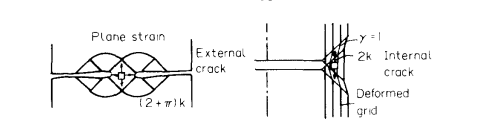
\includegraphics{s5.png}}
    \captionsetup{labelformat=empty}
    \caption{Thickness effect on fracture toughness}
\end{figure}
In order to explain the observed experimental phenomena, it is necessary to resort to the difference
in the state of crack tip stress field. The lower plastic energy dissipation rate in the state of plane strain is
caused by the triaxial state of tensile stress, which causes reductions in effective stress, plastic
deformation, and plastic energy dissipation; and it causes an increase in maximum tensile stress and an
earlier fracture initiation. The data clearly indicate that when the crack tip fields of the effective stress
and the maximum tensile stress change, the fracture toughness will vary.\\\\
Additional evidences of the failure of global energy balance theory are shown by the results of
fracture under combined load. If plastic energy dissipation rate is constant, at the point of fracture
initiation, $(\text{G}_{I} + \text{G}_{II} + \text{G}_{III})$ must be a constant. Experimental evidences have shown that this is far from
universally true [12]. It is evident that if K fails to characterize the same crack tip field, the global energy
balance theory fails to work. Therefore the criterion of global energy balance for fracture initiation
without the consideration of the state of crack tip stresses and the detailed fracture processes, must be
fortuitous. The global energy balance theory is more suitable to the analysis of the final fracture when
the three dimensional effects of crack tip stresses and strains and the associated material responses are
taken into consideration.

\subsubsection{Sharp Notch Analysis}
All crack tips are “blunted,” so sharp notches and cracks can be considered as equivalents. We will
consider sharp elleptical notches in large plates under tensile loading in a direction perpendicular to the
major axis.\\\\
The fracture stress of a notched specimen depends on notch root radius, $R$, as shown schematically
in Figure. $\sigma_c$ decreases with $R$. However, if the notch root radius is less than a certain value $R_c$,$\sigma_c$is no
longer $R$ dependent. When a solid contains a sharp notch of initial root radius $R_i$, the radius increases
with the applied load. If the root radius increment, $\Delta R$ is much larger than $R_i$, the fracture stress $\sigma_c$ is
independent of $R_i$. If the size of the fracture process zone, $\rho_F$ is much larger than $R_i$, $\sigma_c$ will also be
independent of $R_i$. In our analysis, we assume $R$ is always less than $R_c$.

\begin{figure}[H]
    \centering
    \fbox{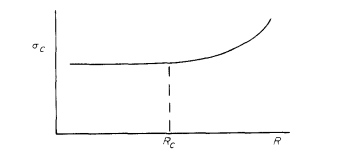
\includegraphics[width=.42\textwidth]{s6.png}}
    \captionsetup{labelformat=empty}
    \caption{Fracture stress as a function of crack tip radius}
\end{figure}

Let us consider geometrically similar elliptical notches in geometrically similar specimens. The major
axis of the ellipse is 2$a$. All the specimens are stressed to the same value of $\sigma_c$. In this case, each
component of $\sigma_{ij}$ or $\epsilon_{ij}$ in all of these specimens has the same value at the geometrically similar points,
$P((r/a), \theta)$. If $\sigma_{ij}$ or $\epsilon_{ij} $control the fracture process and if one specimen fails at a given $\sigma_\infty$ all the
specimens should fail at the same applied stress $\sigma_\infty$, which again contradicts the experimental observations.


\subsubsection{The Theory Of K-characterization}
Under the condition of small scale yielding, SSY, $K$ characterizes the crack tip stresses and strains
even within $r_p$. Let us illustrate this with two samples of different geometry but they are loaded to the
same $K$-value. These samples are made of the same material and have the same thickness
\\\\
Within the region of $r_c(\theta)$ near the cack tip, the singular terms, $\sigma_{ij} = (K/\sqrt{(2 \pi r)} \bar{\sigma}_{ij}(\theta))$
dominate the stress field. $r_e$ is the characteristic elastic crack field zone. For elastic solids, if $r_{e1} = r_{e2}$ the boundary
stresses on $r_{e1}$ and $r_{e2}$ must be equal to each other, since $K_1 = K_2$.
\\\\
In metallic specimens, closer to the crack tip, plastic deformation takes place within $r_p(\theta)$. Let us
examine the regions within $r_{e1}$ and $r_{e2}$ as free bodies given below:
\begin{figure}[H]
    \centering
    \fbox{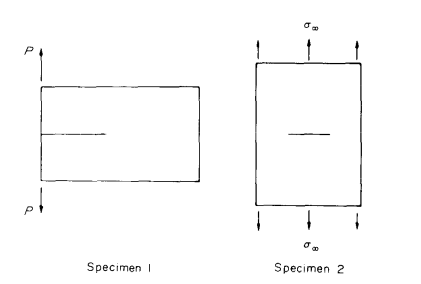
\includegraphics[width=.4\textwidth]{s7.png}}
    \captionsetup{labelformat=empty}
    \caption{Two different fracture toughness specimens, $K_1 = K_2$ }
\end{figure}
In our case, $r_{e1}(\theta) = r_{e2}(\theta)$. If $r_p \ll r_e$ the
stress relaxation within $r_p$ does not disturb much the boundary stresses on $r_e$, therefore, the boundary
stresses on $r_e$ are essentially those given by the singular terms of the linear elastic solution. Since
$K_1 = K_2$, the boundary stresses on these two free bodies must be the same. With the same geometric
shape and size and the same boundary stresses, we must have:

\begin{align*}
    &\sigma_{ij}(r, \theta)_1 = \sigma_{ij}(r, \theta)_2 \\
    &\epsilon_{ij}(r, \theta)_1 = \epsilon_{ij}(r, \theta)_2 \tag{8} \label{8}
\end{align*}
$K_c$ is invariant to planar geometric variation.
 
\begin{align*}
    \begin{array}{@{}c@{}} a\\L \end{array} \geq 2.5 \left( \frac{K_c}{\sigma_c}\right) ^2 \tag{9} \label{9}
\end{align*}
The crack tip $\sigma_{ij}$ and $\epsilon_{ij}$ are not only affected by the planar dimensions of “a” and “L”. They are also
strongly affected by the specimen thickness, t.The size requirements needed to
satisfy the condition of SSY and that of plane strain are
 
\begin{align*}
    \begin{array}{@{}c@{}} t\\a\\L \end{array} \geq 2.5 \left( \frac{K_c}{\sigma_c}\right) ^2 \tag{10} \label{10}
\end{align*}
The condition of $r_e \gg r_p$ is known as the condition of small scale yielding. Wilson has found that
the size of $r_e$ is quite small when compared with other specimen dimensions, only a few per cent of other
planar dimensions of a sample. However, $r_e \propto specimen\ size$; so, in principle, the
condition of SSY can always be satisfied by using a large enough sample. The condition of $r_e$ is a
sufficient but not necessary condition for the validity of the LEFM. The condition could be unduly
restrictive in terms of specimen size requirements. The necessary condition for the validity of the linear
elastic fracture mechanics is that $K$ would be able to characterize the crack tip stress or strain
component at the location of the defined fracture process.

\subsection{Fracture Process Zone}
Materials are inhomogeneous. They contain brittle and ductile phases, inclusion particles, grain
boundaries, etc. Fracture initiation in a cracked solid is often in the interior of a specimen, where the
high tensile stress exists at the locations of brittle and weak materials. Once a local fracture is initiated,
it spreads out. For example, local fracture may start at inclusion 1 (Figure below). The fracture at inclusion I
increases the stress at inclusion 2, and the increased stress causes the fracture of inclusion 2. Ductile
fracture takes place between the brittle particles. If the brittle inclusions are large and closely spaced, it
may cause an avalanche effect, one particle fracturing rapidly after the other. The fracturing process
stops when the crack is out of the zone of the high tensile stress in the plane strain triaxial state of
tension. The crack extension could be sizable and could cause noticeable load drop. This is the well
known phenomenon of pop-in and is a $local\  instability$. Hence, $K_{lc}$ is the result of a local instability
phenomenon, not a global instability.
\\\\
Local fractures may also occur through interface separation between particles and matrix; it may
occur at the embrittled grain boundary, where a high enough tensile stress exists in the plane of the
embrittled grain boundary. The weakened grain boundary may be caused by temper embrittlement,
hydrogen embrittlement, and embrittlement by $\text{O}_\text{2}$, $\text{Cl}_\text{2}$ or other chemicals.

\begin{figure}[H]
    \centering
    \fbox{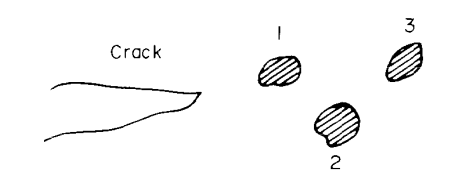
\includegraphics[width=.4\textwidth]{s8.png}}
    \captionsetup{labelformat=empty}
    \caption{Brittle inclusions ahead of a crack tip.}
\end{figure}


Both fracture initiation and stable crack growth are phenomena of local instability. Therefore, the
local energy balance rather than the global energy balance should be used. In order to do so, we need to
treat materials as inhomogeneous substances.
\\\\
The condition of small scale yielding, that enables K to characterize crack tip stresses and strains
responsible for the fracture process, gives the size requirements for the linear elastic fracture mechanics
eqns (9) and (10). In addition, we should impose the condition
\begin{align*}
    \rho_F < r_e \tag{11} \label{11}
\end{align*}
for composite materials. The J-integral removes the requirements for a and L. But an additional size
requirement
\begin{align*}
    \rho_F < r_{cp} \tag{12} \label{12}
\end{align*}
needs to be imposed for metallic fractures. A thickness requirement is also needed for plane strain case.
\subsection{Fracture Toughness And Fracure Ductility}
The initiated local fracture will continue to propagate. The extent of fracture propagation varies
according to the “brittleness” of the material. The fracturing processes can be classified in three
categories.\\\\
(1) Once initiated, the localized fracture will continue to grow rapidly across the specimen without
further increase in $\sigma_\infty$ or $K$. It is very brittle.\\\\
(2) Once initiated, the localized fracture will continue to grow to a sizable extent in a rapid manner
while ($\sigma_\infty$ and $K$ drop. After the initial fracture, it needs to increase $K$ in order to continue to grow
further.
Fracture is initiated in the interior in the plane strain region, and the initial fracturing process will
stop when the crack is out of the zone of triaxial state of tension.
\\\\
(3) If fracture initiation is caused by brittle particles and if the brittle particles are small and far
apart, once the local fracture is initiated, it needs a considerable amount of plastic deformation to grow
across the regions between particles. A crack grows primarily by the process of plastic deformation.
This material is ductile and tough.
\begin{figure}[H]
    \centering
    \fbox{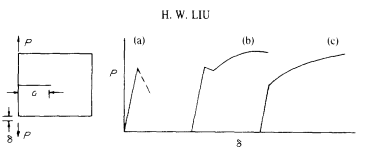
\includegraphics[width=.5\textwidth]{s9.png}}
    \captionsetup{labelformat=empty}
    \caption{Schematic diagrams of load vs load point displacement showing difference in fracture ductility}
\end{figure}
$K$ and $J$ characterize $\sigma_{ij}$ and $\epsilon_{ij}$ within the fracture process zone. The maximum tensile stress, $\sigma_{\text{max}}$,
could be the parameter that controls fracture initiation in the case of brittle particles, The nucleated
crack may then propagate rapidly for a clear definition of $K_{lc}$. as shown in Fig. (a) and (b). In this
case, $K_{lc}$ might be correlated with $\sigma_{\text{max}}$. On the other hand, if the particles are small and far apart, the
nucleated minute local fractures will grow by a mechanism which needs a great deal of plastic
deformation. If $K_{lc}$ is defined by a specific amount of crack growth, primarily by a mechanism of plastic
deformation, $K_{lc}$ will be correlated better with the effective plastic strain, $\bar{\epsilon} ^ p$. If a crack propagates by
the shear-off process between the ductile matrix and hard second phase, then the maximum shear strain
should be used. The beauty of both of the linear and non-linear fracture mechanics, is that both the $K$
and $J$ can be used in all of the illustrated cases, because $K$ and $J$ characterize all the stress and strain
components, as well as their combinations such as $\bar{\sigma}$, $\sigma_{\text{max}}$, $\bar{\epsilon} ^ p$, $\gamma_{\text{max}}$, and strain energy density if the
condition of $\rho_F < r_{cp}$is satisfied.
\\\\
$K$ and $J$ are macro-parameters. As long as they can characterize the stresses and strains at the
location of fracture initiation and fracture propagation, they can be used to measure fracture toughness
regardless of the details of the initiation and propagation processes. Clearly, we use $K$ and $J$ as indirect
parameters which do not infer any specific fracture process.
\\\\\rule{\textwidth}{.1em}



%------------------------------------------------------------------
%------------------------------------------------------------------
\section{Computational Fracture Mechanics}
This topic focuses on the impact of computational methodology on furthering the understanding of fundamental fracture phenomena. The current numerical approaches to the solution of fracture
mechanics problems, e.g. finite element (FE) methods, finite difference methods and boundary element
methods, are reviewed. The application of FE methods to the problems of linear elastic fracture problems
is discussed. A special focus is placed on stable crack growth problems. The need for further research in this
area is emphasized. The importance of large strain phenomena and accurate modelling of non-linearities
is highlighted. An expanded version of fracture mechanics methodology is given by Liebowitz \textit{[Advances  in Fracture Research 3. Pergamon Press, Oxford (1989)]}; additional treatment is given in this paper to
numerical results incorporating error estimates and algorithms for mesh design into the FE code. The
adaptive method involves various stages which includes FE analysis, error estimation/indication, mesh
refinement and fracture/failure analysis iteratively.

%------------------------------------------------------------------
\subsection{Numerical Methods For Solution Of Fracture Problems}
The problems of fracture mechanics reduce to the solution of boundary value problems (which may
be static or dynamic) which have mixed boundary conditions. The shape and the mixed boundary
conditions can give rise to singularities in the stress and strain fields. The problems may involve
both material and geometric non-linearities, which complicate the formulation and render
prediction of convergence extremely difficult. Because little can be done with these problems
analytically, numerical methodologies are required.
\\\\
The \textit{finite difference} method is the oldest technique for the solution of boundary value
problems. The method directly involves the solution of the
governing differential system in an approximate manner by subdividing the domain of interest into
a connected series of discrete points called nodes. These nodes are the sampling points for the
solution and are linked using the finite difference operators to the governing equations. Employment 
of the finite difference operators results in a system of algebraic equations for the discrete
nodal values of the field variable. The finite difference method can be used to discretize both space
and time. The finite difference method is difficult to use for irregularly shaped domains or for problems involving
singularities, because the fine meshing required near a singularity cannot easily be reduced for the
rest of the domain. 
\\\\
\textit{Integral equation methods} basic approach employed involves an analytic formulation
of the elasticity problem to the point of a singular integral equation. The singularity is then
extracted and the result is a non-singular integral equation which can be solved quite accurately
with any number of techniques. This approach yields excellent solutions; however, it requires an
extensive analytic formulation which is different for each new problem. The method is quite useful,
nonetheless, for establishing benchmark solutions to compare with other methods as the degree
of accuracy can be guaranteed. The method is only applicable to elasticity problems (without
non-linearities). For three-dimensional problems, the derivation of the integral equations becomes
quite laborious.\\\\
The \textit{Boundary Integral Equation  Method} (BIEM) is a numerical approach to the solution of
linear boundary value problems with known Green's function solutions. The boundary of the
domain of interest is discretized using "elements" which are interconnected at discrete points called
nodes. For a three-dimensional problem, the mesh is two-dimensional; for two-dimensional
problems, the mesh is one-dimensional. The boundary value problem is formulated as an equivalent
surface or line integral using the Green's function solution and the governing differential system.
For linear elasticity in two dimensions, the formulation is based on Betti's theorem and the resulting
system of equations is given by
\begin{align*}
    C_{ij}u_j + \int_{\varGamma} T_{ij}u_j  \,d\varGamma + \int_{\varGamma} U_{ij}t_j  \,d\varGamma \tag{13} \label{13}
\end{align*}

where $U_i$ and $t_i$ are the surface displacement and traction vectors on the domain boundary, and
$U_{ij}$ and $T_{ij}$ are related to the Green's function solutions for displacements and tractions,
respectively. At each boundary point, either $u_j$ is specified (on $\varGamma_u$) or $t_j$ is specified on ($\varGamma_t$), while
the variable is unknown.
For static problems, the BIEM
reduces to the solution of a system of dense linear equations which may be non-symmetric. If
surface data are the only quantities required,the BIEM is often
computationally superior to the FEM for two-dimensional problems. If interior data are required,
the method is computationally costly. For three-dimensional problems, BIEM solutions are often
very expensive as the resulting linear system is dense, unbanded and often non-symmetric, and often
do not produce good solutions.
\\\\
The \textit{Finite Element Method} is the most widely employed numerical method for fracture mechanics problems.
The formulation of the FEM is based on a variational statement of the governing physics. For the
problems of linear elasticity, the Principle of Virtual Work, given by
\begin{align*}
    \int_{v}\sigma_{ij} \delta \epsilon_{ij} \text{d} V = \int_S \sigma_{ij} n_j \delta u_i \text{d} S \tag{14} \label{14}
\end{align*}
which is employed, where $\sigma_{ij}$ is the stress tensor, $\delta \epsilon_{ij}$ is the virtual strain tensor due to virtual displacements
$\delta u_i$ and $n_j$
is the normal vector to the surface of applied tractions. The domain is discretized into
subdomains (elements) which are interconnected through common discrete points (nodes). The
primary unknown field variables are nodal values. The formulation reduces the problem to the
solution of a system of algebraic equations in terms of the nodal variables (for dynamic problems,
the result is a system of ordinary differential equations). Finite element systems tend to be relatively
banded and symmetric for most problems.For fracture mechanics problems, the FEM can be employed in the standard manner or
modified to account for the singular nature of the near crack fields.


\begin{center}
    \begin{tabular}{ l l l } 
     \hline
    \\Method             & Strengths &weaknesses\\\\ \hline
    \\Finite difference   & $\begin{array}{@{}l@{}} \text{Easy to employ}\\\text{Error estimates available} \end{array}$& $\begin{array}{@{}l@{}} \text{Slow convergence}\\\text{Uniform mesh requirement} \\\text{Cannot model singularities}\end{array}$ \\\\\hline
    \\Finite elements    & $\begin{array}{@{}l@{}} \text{Good convergence}\\\text{Singularities can be modeled} \end{array}$ &  $\begin{array}{@{}l@{}} \text{Modeling is difficult}\\\text{Few existing error estimators} \end{array}$ \\\\\hline
    \\Boundary element   & $\begin{array}{@{}l@{}} \text{Modeling is easier}\\\text{Error estimation is easy} \end{array}$ &$\begin{array}{@{}l@{}} \text{computationally more expensive }\\\text{Converges slowly for singular problems} \end{array}$\\\\\hline
    \\Hybrid approaches  & $\begin{array}{@{}l@{}} \text{Good for specific problems}\\\text{Generally very accurate} \end{array}$& $\begin{array}{@{}l@{}} \text{Usually developed for restricted problem class}\\\text{difficult to implement} \end{array}$\\ 
     \\\hline
    \end{tabular}
\end{center}
%-----------------------------------
\subsection{Impact Of FEM On LEFM}
\subsubsection{Stress Intensity Factors}
The ability to predict accurately the stress intensity factors for cracked elastostatic bodies using
standard numerical techniques has greatly advanced the use of LEFM concepts in application.
Most commercial
FEM and BIEM codes have two-dimensional elastostatic fracture capabilities built-in and
automated.
\\\\
The prediction of three-dimensional stress intensity factor distributions is not a straightfor-
ward process. Research in this area has been ongoing for more than 10 years. Special singular
elements have been proposed by Tracey , Blackburn and Hellen, Hilton and others. These
singular elements are based on employment of the asymptotic displacement field in the finite
element formulation directly. The element geometry is the same as the corresponding standard
elements. As analyzed elsewhere, these approaches require the assumption of a local state
of plane strain near the crack front which has not been established analytically. They must be
utilized, therefore, with discretion.
\\\\
Once the FE field solutions are obtained, there are essentially two approaches to calculate the
stress intensity factors: the multi-term displacement field approach and the nodal force
approach. These approaches are based on the asymptotic displacement field and stress field
near the crack front, given as
\begin{figure}[H]
    \centering
    \fbox{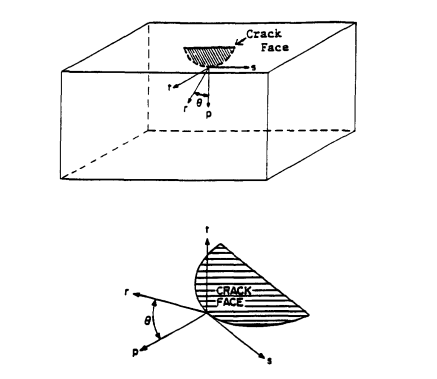
\includegraphics[width=.55\textwidth]{s10.png}}
    \captionsetup{labelformat=empty}
    \caption{Three-dimensional crack geometry.}  
\end{figure}


\begin{align*}
    &u_{1}^{1} = \left(\frac{1 + \nu}{E}\right)\left(\frac{2r}{\pi}\right) ^{1/2} \left\{K_I\cos\frac{\theta}{2}\left[(1-2\nu)+\sin ^ 2 \frac{\theta}{2}\right] + K_{II}\sin \frac{\theta}{2}\left[2(1 - \nu) + \cos ^ 2 \frac{\theta}{2}\right]\right\}\\
    &u_{2}^{1} = \left(\frac{1 + \nu}{E}\right)\left(\frac{2r}{\pi}\right) ^{1/2} \left\{K_I\sin\frac{\theta}{2}\left[2(1-\nu)+\cos ^ 2 \frac{\theta}{2}\right] - K_{II}\cos \frac{\theta}{2}\left[2(1 - \nu) + \sin ^ 2 \frac{\theta}{2}\right]\right\}
 \\ &u_{2}^{1} = 2\left(\frac{1 + \nu}{E}\right)\left(\frac{2r}{\pi}\right) ^{1/2} K_{III}\sin \frac{\theta}{2} \tag{15} \label{15}\
 \\&\sigma_{ij} = \frac{K_{I}}{\sqrt{r}}f_{ij}(\theta) + \frac{K_{II}}{\sqrt{r}}g_{ij}(\theta) + \frac{K_{I}}{\sqrt{r}}f_{ij}(\theta) + \frac{K_{III}}{\sqrt{r}}h_{ij}(\theta) \tag{16} \label{16}
\end{align*}


where$ f_{ij}, g_{ij}$ and $h_{ij}$ are known functions of $\theta$; the local coordinate system is defined.
It should bementioned that, due to the assumption of local plane strain in the neighborhood of the crack front,
the multi-term displacement method can yield erroneous results where crack front curvatures are
large or as the crack front approaches a free surface.

\subsubsection{Energy Release And J-integral}

The Griffith energy release theory of LEFM is widely accepted as a criterion for fracture proof
design. This theory involves the calculation of the amount of energy released with a virtual
extension of the crack. The criterion originally proposed by Griffith requires that the crack can
be idealized as a line of discontinuity and that the remote loading is tensile and normal to the crack.
In other words, it is restricted to a two-dimensional linear, elastic mode I fracture problem. In such
a case, it is well known that the energy release rate can be related to the stress intensity factor $K_1$
and the path independent $J$-integral as follows:

\begin{align*}
    G = J = \pi (\kappa + 1 ) K_{I}^{2}/ 8 \mu \tag{17} \label{17}
\end{align*}

where $\kappa = 3 - 4 \nu$ for plane strain and $\kappa = (3 - \nu)/(1 + \nu)$ for generalized plane stress;
the $J$-integral is defined as
\begin{align*}
    J = \int_\varGamma (U \text(d)y - \sigma_{ij} n_j u_{i, x}\text{d}s) \tag{18} \label{18}
\end{align*}

For two-dimensional mixed mode fracture problems, if the crack is to extend along the line
of the crack, i.e. self-similar crack extension, then the $G - J - K$ relation is given as
\begin{align*}
    G = J = \pi (\kappa + 1)(K_{I}^{2} + K_{II}^{2})/8\mu \tag{19} \label{19}
\end{align*}
If the line of crack extension deviates from the crack line by an angle $\theta$, then the energy release
rate is obtained as
\begin{align*}
    G(\theta) = \pi(\kappa + 1)(1 + c)[K_{1}^{2}(1+c) + K_{11}^2(5-3c)-4K_{1}K_{11}s]/32\mu \tag{20} \label{20}
\end{align*}
It is emphasized that the energy release rate theory originally proposed by Griffith is now
generalized; eq. (20) is the general $G - K$ relation; the value of $G_{max}$ is greater than that of $G$ obtained
from eq. (19) for self-similar crack extension; and $G_{max}$ is greater than the value of the $J$-integral
and hence it is fair to say that the $J$-integral is only applicable to self-similar crack extension
problems.
\subsubsection{Dynamic Crack Propogation}
In addition to the study of static LEFM problems, much work has been performed for
dynamic LEFM problems. In the dynamic case, two problems are important: that of a running
crack and that of a static crack with elastic waves impinging. The problem of stress intensity factor
calculation for static cracks in elastic materials subjected to time-dependent loading is no more
difficult than the corresponding static problem. The same solution methodologies are employed and
the results can be calculated to the same accuracy. Computational requirements are greater;
however, no new problems arise numerically. The problem of a running crack in an elastic material
is much different from the problem of a static crack. FEM solutions have had a major impact on
this area. Few analytic solutions to realistic problems are available (even in two dimensions);
therefore, robust numerical approaches are essential. The first realistic solution to the problem of
a running crack was presented by Anderson. They introduced a nodal release algorithm
which models the changing boundary conditions of a growing crack. The method has proved to
be very robust and easy to implement, even in commercial finite element codes, and is widely
employed. This algorithm has allowed many researchers to study running crack problems for a wide
variety of geometries and loadings.  An interesting example of dynamic crack propagation
simulation involves the problems of interacting cracks. Consider the problem of two cracks in a
sheet which are opened by wedge loads. The cracks at two sides of the sheet are slightly
misaligned to provide initial asymmetry. Figure shows the cracks at three stages of the analysis.
Initially, the cracks repel each other and, as propagation continues, they attract. At the final stage,
the two cracks intersect. Figure shows the stress intensity factor histories as a function of crack
length. The positive mode II component is evident during the avoidance stage and negative mode
II is evident during attraction.


\begin{figure}[H]
    \centering
    \fbox{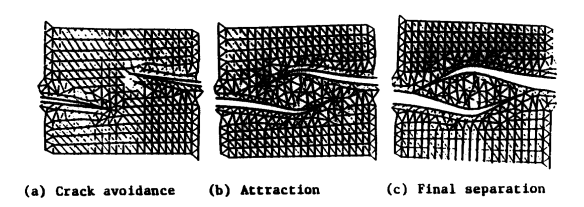
\includegraphics[width=.9\textwidth]{s11.png}}
    \captionsetup{labelformat=empty}
    \caption{Displacement plots during crack propagation}  
\end{figure}

\subsection{Adaptive Finite Element Analysis}
One of the biggest problems with finite element analysis (FEA) lies in the fact that an
assessment of the reliability of the FE solution is difficult to obtain. The FE
analyst is usually guided by experience in designing and assessing the quality of the mesh. After
solution, simple checks, such as examining the stress discontinuities between elements, can be made
to assess the quality of the solution. Based on the analyst's experience the solution is accepted or
rejected. If this approach can be automated, not only would the solution be improved but a large
saving in man-hours would be made.
\\\\
The projection or stress smoothing type error estimators are a global measure of the
discretization error contained in any given FEA. For adaptive schemes the local error does tend
to approach the global (average) error in an iterative fashion. The basic idea of these estimators
is that an approximation of the error due to the mesh discretization can be made given the FEA
solution and an appropriate better approximation to the continuous stress solution. Adaptive mesh
generation can be approached in a variety of ways, the two most common being the h- and
p-versions. The h-version improves the accuracy of the solution by refining the mesh, while the
p-version uses a fixed mesh but increases the polynomial degree of the shape functions. In the
present work the projection type error estimators combined with h-version mesh refinement
algorithms which use quadrilateral elements are investigated for two-dimensional linear elastic
problems. The mesh refinement algorithms are based on simple and hierarchical schemes
for subdividing quadrilaterals with transitioning, which avoids the need for constraint equations
to enforce compatibility at element boundries. Another scheme is based on using constraint
equations to enforce compatibility between elements. This h-version will not have as high a
convergence rate as a combined h-p-version (or even a p-version), but the h-version is easier to
program and the results are easier to interpret,
\\\\\rule{\textwidth}{.1em}
\section{Probabilistic Fracture Mechanics}
The interest in applying statistics to assess structural reliability has continued to
increase. This is evident from the large amount of work in
probabilistic fracture mechanics (PFM) and associated topics.
Many factors contribute to reliability and these often change both systematically
and at random. In the past, structures have been designed using a simple factor of
safety approach to calculate a safe lifetime over which the applied loads will be
sustained. Each variable in the equations governing the operation of the system was given a reasonable
value drawn from past results or even just human intuition, and a predicted life
obtained. This was then divided by a factor of safety which reduced it to give a 'safe'
maximum operating life. It is conceivable that this is unrealistically conservative but simple.\\
So that there is a demand,
particularly from industry, for a statistical justification behind the calculations,
since many parameters may influence the behaviour of a structure and in practice
each will be subject to both random and systematic variations.\\\\
One approach is to use historical data from past failures and non-failures to
evaluate the reliability of current productions.\\\\
Thus, an alternative approach has been sought, namely the development and
application of engineering models based on an understanding of the failure modes
and statistical distributions of the controlling parameters. The latter distributions
are not always known, so that errors may be introduced because of poor
assumptions.\\\\
Ideally, a combination of the two methods is necessary so that past experience
and results plus specially designed laboratory tests can be used to obtain statistical
distributions which best fit these data, but also, hopefully provide predictions about
altered or new systems. The problem is then divided:\\\\
{\it 1. The basic problem:}
The two main considerations are the distribution of crack-like defects (or flaws)
introduced during the fabrication of a structure and the critical crack length
distribution for the material under service conditions, the latter being controlled
primarily by the fracture toughness.In general, there is a lack of data for
the initial distribution of defects in a structure so the distribution is often assumed to
be lognormal or exponential. From a failure point of view, it is importanl to know
how this distribution compares with that of the critical crack size, which is
controlled by the material properties, and applied loading. The probability of
failure is then given by the probability of interaction of the actual crack or flaw $a_i$,
and a critical crack length $a_{c}$\\\\
In the above, there has been an inherent assumption of independence between $a_i$
and $a_c$. Marriott and Churchill pose a warning that the presence of defects in
regions of low toughness material may potentially increase the failure probability by
several orders of magnitude. A preliminary examination of service failures suggests
the possibility of a correlation effect may indeed be a real one, not to be ignored.\\\\
{\it 2. Further considerations: }Closely linked with the as-fabricated flaw size distribution is the role played by
non-destructive testing in detecting defects which may, or may not, be repaired.
Thus, if the initial flaw distribution and the probability of detecting a defect are
known, then the distribution of flaws when the structure is put into service can be
deduced.\\\\        
In situations where fatigue cracking occurs, the defect distribution will tend to
alter with the number of applied cycles.This
problem may be reduced by in-service inspection at fixed intervals of time, and by
repairing the defects so found.
\subsection{General}
The concept of design factors can be pursued in the probabilistic models where the
factors themselves are defined in terms of the ratio of characteristic values of load
and strength based on statistical models of the variables instead of the mean values.
For example, the characteristic value for load may be the 90 percentile value of the
load distribution and for strength the 5 percentile value of the strength distribution.
(Here, '90 percentile value' indicates the value below which a load is expected to fall
with 90\% confidence.) The optimisation of the inherent cost may also be included.
Alternatively, the uncertainties of the different loads may be combined statistically, 
since only one safety factor should be sufficient since there is just one design
condition, namely the specified reliability level.\\\\
Other approaches include fault tree analysis which is essentially a deterministic
approach whereby each event in a sequence is assigned a probability of success/
failure. Fukuda considers this as a link between probabilistic and qualitative
methods and explains its use with respect to improving the reliability of welded
structures. However, no distribution functions are assumed and so there can be no
real consideration of the uncertainties involved. The component probabilities are
assumed known, though they may be ill-defined.\\\\
In the probabilistic treatment, the random variations are described using
distributions of values for the parameters rather than one deterministic value. The
distribution may be thought of as a curve combining the possible values and the
likelihood (probability) they will occur. The introduction of distributions of values
necessarily complicates an analysis, but the end result is likely to be more accurate
and hence of more use. In some cases, neat analytical expressions for the reliability
are impossible and numerical approximations are required. 
Approximate interactive algebraic procedures are used to determine an estimate of
the failure probability ( = 1 - reliability), whereas in the latter, the approximation is
at a later stage, after all the exact probabilistic expressions have been obtained for
the complete system; this ibe justified by the improvement gained.s, of course, much harder, and the work involved may not be justified by the improvement gained.
\subsection{Statistical Basis Of PFM}
The basis of PFM is the simple axiom that a given
mode of failure event E will occur when the stress $\sigma_w$
associated with the failure mode exceeds the mode
governing strength $\sigma_f$. The probability of failure mode
$E$ is given by
\begin{align*}
    \text{P}(E) = \text{P}(Y < 0) = \text{PD}(y=0)\\~\\
    \text{where the strength margin, }
    Y = \sigma_f - \sigma_w = G(x_i)
\end{align*}
with $i = 1 ..... n_x$, depends on input variables that at affect component stress or strength or both. An alterna-
tive definition in terms of a strength ratio $Y = \sigma_f/\sigma_w$
is equally valid and leads to P($E$) = P(($Y$)< 1)
\begin{figure}[H]
    \centering
    \fbox{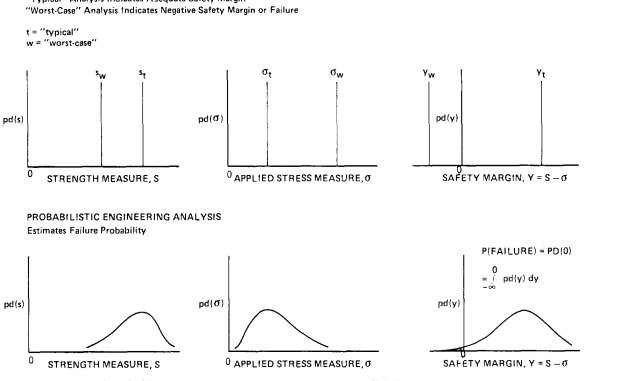
\includegraphics[width=.6\textwidth]{s13.png}}
    \captionsetup{labelformat=empty}
    \caption{Fig.(a)Contrast between deterministic and probabilistic engineering analysis.}  
\end{figure}
\begin{figure}[H]
    \centering
    \fbox{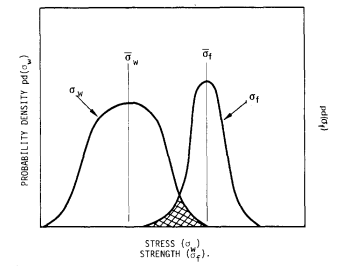
\includegraphics[width=.4\textwidth]{s14.png}}
    \captionsetup{labelformat=empty}
    \caption{Fig.(b)Statistical variation of strength ($\sigma_f$) and applied stress ($\sigma$); failure possible over crosshatched region.}  
\end{figure}

Here, $G$
is a concise deterministic summary of all prior engineering experience, models, and assumptions. If the
engineering analysis does not lead to an obvious functional 
form, $G$ may be obtained from standard least-
squares fitting of the engineering data or by the repetitive
 analysis procedure.the $x_i$ are most realistically described as ran
dom variables $X_i$ rather than single assigned deterministic values. 
As shown in fig.(a), statistical interpretation 
of the $X_i$ results in the interpretation of
strength margin as a random variable. The statistical
interpretation also allows the analyst to quantify his
uncertainty of the engineering model $G$ based on
judgement, and his previous record of predictive suc-
cess and failure. This error quantification is done by
introducing one or more additional $X_i$ to serve as
'error terms'.
The cumulative distribution functions of the $X_i$,
represented by\\\\
\begin{center}
    PD($x_i$) = P($X_i \le x_i$)
\end{center}

\subsection{Flaw Distribution}
Perhaps the greatest problem in assessing the reliability of a welded structure is that
of data on defects which may be present. Ideally, there should be no defects, but in
practice no structure is completely defect free, since no-one is perfect and the result
can only be as accurate as the tools available permit, including the experience (or
lack of experience) of human operators involved.\\\\
In terms of fracture mechanics it is the crack depth that is of
importance. Fearnehough and Jones present such data for seamless and seam
welded pipe, estimated from preservice pressure test failures. In recent years pipe
supplies have been remarkably improved in quality, so alternative information has
been obtained by sectioning and measuring all detected defects in a sample of nearly
3000 seamless pipes. The data are similar to those from the failure analysis, but still
do not represent the true defect population of an existing pipeline since some defects
may have been missed in the inspection and the pressure test will eliminate large
unacceptable defects and some smaller insignificant ones.\\\\
A way of helping to solve the problem of missing defects is described by Jagger
and Manning. The largest defect in each weld is recorded and an extreme value
distribution used to model these data. From this, predictions may be made
regarding the behaviour of the largest defects, which are expected to be most
damaging. Weld defects found in high Temperature steam pipe welds by non-
destructive testing (NDT) techniques are analysed in terms of the defect length and
depth through the wall thickness to obtain the appropriate distributions.
\subsection{Non-Destructive Testing(NDT)}
After fabrication, a structure is usually inspected to check for large 'unacceptable'
flaws which require repair before service. This inevitably changes the initial defect
distribution by filtering some of the larger defects. A general appreciation of NDT is
given by Hansen including some of the difficulties encountered. No technique of
non-destructive inspection is perfect, so that a probability of detection is associated
with each, and this may well vary according to the defects of interest. In terms of
fracture mechanics analysis the defect depth is essential, so that an estimate of the
accuracy of sizing capabilities must be determined.
Packman investigated penetrant systems of aluminium and titanium,
which yield greater than 90\% ability to detect surface cracks of length greater than
0.939 mm. The probability of detection decreases for small cracks and also varies in
accuracy depending on the inspectors' capabilities. Although two may find the same
total number of defects (i.e. the same detection probability) one may have a higher
percentage of false indications.
So, defect detection probability, DDP, is used:
\begin{align}
    \text{DDP}=\frac{\text{Number of teams successfully detecting a particular defect}}{\text{Total number of teams}}
\end{align}
\subsection{Material Properties}
Swindeman claims that he has found that variability
in material properties can be traced to differences in chemistry, fabrication and
testing procedures. These correlate well with heat-to-heat, product-to-product and
laboratory-to-laboratory variability, respectively.\\\\
In structures where target failure probabilities are low, it is the extremes of the
distributions that are of interest, including the possibility of inconceivable events
producing 'outliers' to the distribution.

\subsection{Fatigue}
Failure by fatigue is a common occurrence in welded joints. Small cracks at weld
toes (or the root) may propagate under cyclic loading.It is usually assumed that the stress range versus endurance (S-N) curve is a
straight line with two parallel lines. For a particular stress level, S, it is the
scatter in fatigue life, N, that is of interest. Therefore, a probability density function
for N is required.
\begin{figure}[H]
    \centering
    \fbox{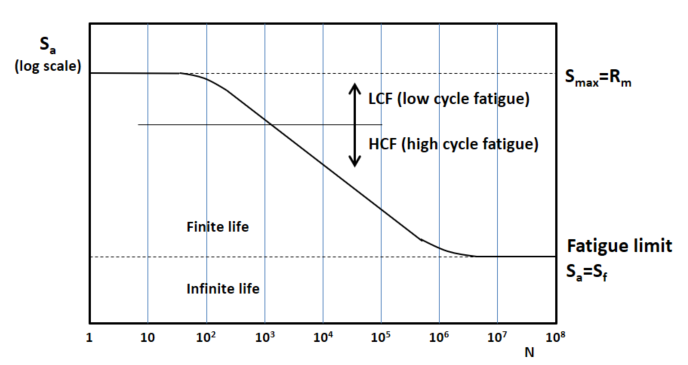
\includegraphics[width=.6\textwidth]{s12.png}}
    \captionsetup{labelformat=empty}
    \caption{General S-N curve}  
\end{figure}
\subsection{Mathematical Techniques}

The problem of obtaining sufficient data, upon which statistical predictions for a
component may be based, is a real one. Where previous information is available,
estimates of sample size may be made using the (previous) sample standard
deviation. However, more often, there are no data readily
available. Either a guess must be made for the expected variance of the results or
sequential testing may be utilised. Smith explains how the method is based on the
desired and minimum acceptable reliabilities and the risk involved. After each test,
the number of failures and successes is reviewed and a decision made to accept or
reject the component or to continue sampling. In general, even when the sample size
can be estimated, fewer tests are required using sequential testing.
An approximation to the amount of confidence which can be placed in the
minimum of a small sample of results is given by Wilks. The equation:
\begin{align*}
    \beta^n = 1 - \alpha
\end{align*}


predicts the percentage, $\beta$, of data (from the population) which would be expected to
lie above the minimum of n sample results with a confidence of $\alpha$
\\\rule{\textwidth}{.1em}
\section{Probabilistic fracture mechanics by using Monte Carlo simulation
and the scaled boundary finite element method}
In PFM, the sensitivity of the stress intensity stresses are more often than not required to predict the 
reliability or probability of fracture initiation. 
Early works in this area include that of which examines probabilistic analysis techniques to estimate the reliability
 of various response variables, such as the SIF, on the basis of its sensitivity to randomness or uncertainty in the
input variables. Commonly used techniques include the Monte Carlo simulation (MCS) method and the first-order reliability
method (FORM). For both methods, uncertainties in the applied load, material properties, and crack geometry are modeled
as random variables described by specific probability distribution functions. In the MCS methodology, these random
variables are generated many times from its distribution function. For each of the Monte Carlo samples, the SIFs, which
are sensitive to the randomness of the variables, are computed. The resulting SIFs are compared with the material toughness
to evaluate whether failure will occur. Certainly, many deterministic evaluations need to be performed for the MCS method.
The method can also be combined with other techniques of fracture modeling such as cohesive elements to perform a
reliability analysis. On the other hand, the FORM method requires the mathematical derivative of the SIFs. Evaluation is
based on solving an algorithm, such as the Hasofer and Lind algorithm, to linearly approximate the most probable point
of failure. Subsequent studies that exercise these procedures. In all of these
studies, the sensitivity of the SIF with regards to uncertainties in the applied loads and material properties are shown to be
dealt with easily.\\\\the scaled boundary finite-element method is employed to investigate the shape sensitivity of the stress
intensity factors of a crack to the size and orientation of the crack. Only a single boundary mesh is required. The variation
of the crack size and orientation can be represented by simply changing the position of the crack tip without the need for
remeshing the boundary. Therefore, the repetitive deterministic analysis is made simple, elegant, and highly efficient as
compared to most other numerical methods. Thus, it becomes feasible to use the brute force MCS method for the reliability
analysis of a cracked structure.
\subsection{Scaled Boundary Finite Element Method(SBFEM) For Shape Sensitivity Analysis}
\subsubsection{Summary of the scaled boundary finite element method for fracture analysis}A 2D homogeneous domain containing a crack tip is illustrated in Figure. The geometry of the domain satisfies the scaling
requirement, i.e., the whole boundary of the domain is directly visible from the crack tip. Problems of more complex 
geometry can be divided into such smaller subdomains.
The scaling center O is selected at the crack tip.
Without loss of generality, the origin of the Cartesian coordinates $\hat{x}$ and $\hat{y}$
is defined at the scaling center. The boundary is discretized with line elements. The nodal coordinates at the boundary
are denoted \{$x$\} and \{$y$\},
with shape functions [$N( \eta )$] in the local coordinate $\eta$ . Thus for any point on the boundary the Cartesian 
coordinates ($x, y$), can be interpolated by 
\begin{align*}
    x = [N(\eta)]\{x\}\\
    y = [N(\eta)]\{y\} \tag{21} \label{21}
\end{align*}
\begin{figure}[H]
    \centering
    \fbox{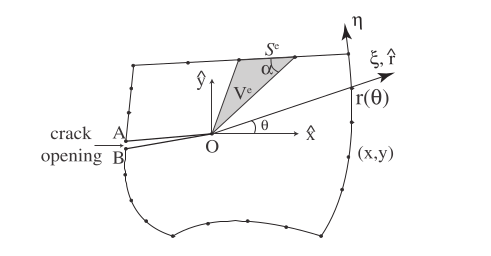
\includegraphics[width=.4\textwidth]{s15.png}}
    \captionsetup{labelformat=empty}
    \caption{2D cracked plate in scaled boundary coordinate}  
\end{figure}

The domain is generated by scaling the boundary along the radial coordinate $\xi$ 
pointing from the scaling center O to a point
on the boundary. In other words all such boundary line element segments
$S^e$ are scaled to the scaling cemter O to form such and area $V^e$. By using eq. (21), the coordinates of any point within the domain $(\hat{x}, \hat{y})$
can then expressed as:
\begin{align*}
    \hat{x} = \xi x = \xi [N(\eta)]\{x\};\\
    \hat{y} = \xi y = \xi [N(\eta)]\{y\}; \tag{22} \label{22}
\end{align*}

where the scaling factor $\xi$ takes the value of 0 at the scaling center and 1 on the boundary. $\xi$ and $\eta$ are called the scaled
boundary coordinates. To reiterate, the coordinates of a point in the domain are denoted as $\hat{x}$ and $\hat{y}$ while $x$ and $y$ are researved
for the boundary. Note that the two crack faces OA and OB are formed by scaling Points A and B, and thus are not
discretized, a distinguishing attribute of the SBFEM for fracture applications.
The Jacobian of the coordinate transformation  is expressed on the boundary ($\xi = 1$) as
\begin{align*}
    [J(\eta)] = \begin{bmatrix}
        x & y\\
        x.\eta & y.\eta 
    \end{bmatrix}
\end{align*}

To avoid the Jacobian of the
scaled boundary coordinate transformation approaching zero, the acute angle formed by a radial line and the boundary should not be too small.
As shown in Figure below for a single 2-node element, nodal displacement functions {$u(\xi)$} are introduced along the radial lines
passing through the scaling center O and a node on the boundary. Along the circumferential direction $\eta$ , the displacements is
obtained by interpolating the nodal displacement functions

\begin{align*}
    \{u(\xi, \eta)\} = [N(\eta)]{u(\xi)}
\end{align*}


\begin{figure}[H]
    \centering
    \fbox{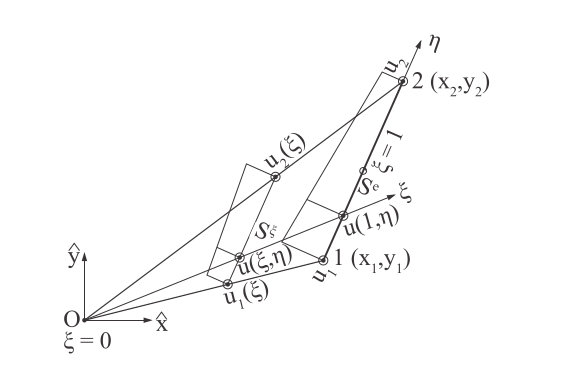
\includegraphics[width=.4\textwidth]{s16.png}}
    \captionsetup{labelformat=empty}
    \caption{Displacement in scaled boundary coordinates}  
\end{figure}

Applying a weighted residual technique in the $\eta$ direction leads to the following scaled boundary finite element equation in displacement
\begin{align*}
    [E^O]\xi^2\{u(\xi))_{,\xi\xi} + ([E^0] - [E^1] + [E^1]^T)\xi\{u(\xi)\}_{, \xi} - [E^2]\{u(\xi)\} = 0 \tag{23} \label{23}
\end{align*}

The global coefficient matrices $[E^0], [E^1 ] $and $[E^2 ]$ are obtained by assembling the element coefficient matrices over the 
complete boundary in the same manner as for the stiffness matrices in the finite element method. The element coefficient 
matrices are given by
\begin{align*}
    [E^0] = [B^1(\eta)]^T[D][B^1(\eta)]|J(\eta)|d\eta;\\
    [E^1] = [B^2(\eta)]^T[D][B^1(\eta)]|J(\eta)|d\eta; \tag{24} \label{24}\\
    [E^2] = [B^2(\eta)]^T[D][B^2(\eta)]|J(\eta)|d\eta; 
\end{align*}


where $[D]$ is the elasticity matrix. where $[B^1(\eta)]$ and $[B^2(\eta)]$ describe the strain-displacement relationship with

\begin{align*}
    [B^1] = \frac{1}{|J|} \begin{bmatrix}
        y,\eta & 0\\
        0 &-x,\eta\\    
        -x,\eta & y,\eta
    \end{bmatrix}
    [N(\eta)]
\end{align*}

\begin{align*}
    [B^2] = \frac{1}{|J|} \begin{bmatrix}
        -y & 0\\
        0 &x\\    
        x & -y
    \end{bmatrix}
    [N_{,\eta}(\eta)]
\end{align*}
The displacement functions {$u(\xi)$} are expressed as
\begin{align*}
    u(\xi) = \sum_{ i = 1}^{N-1} [\varPsi_{i}^{u}]\xi^{-[S_i]}\{c_i\} + [\varPsi_{N}^{u}]\{c_N\} \tag{25}
\end{align*}


where $[S_i](i = 1, 2, . . . , N)$ are diagonal blocks of the real Schur matrix, [$\varPsi _{i}^{(u)}$] the corresponding displacement modes and {$c$}
integration constants, which are determined from the displacements on the boundary {$u(\xi = 1)$}. As in the finite element
method, stresses are evaluated element-by-element, yielding the values at a specified local coordinate $\eta$ within a given
element
\begin{align*}
    \{\sigma(\xi, \eta)\} = \sum_{i = 1}^{N-1}[\varPsi_{\sigma i}(\eta)]\xi^{-|S_i| - |I|}\{c_i\} \tag{26}
\end{align*}

where $[\varPsi_{\sigma i}(\eta)]$ represents the stress modes corresponding to the displacement modes [$\varPsi_{i}^{(u)}$]
\begin{align*}
    [\varPsi_{\sigma i}(\eta)] = [D](-[B^1(\eta)][\varPsi_{i}^{(u)}][S_i]+[B^2(\eta)][\varPsi_i^{(u)}]) \tag{27}
\end{align*}
\\\\
\subsubsection{Evaluation of stress intensity factors}
When the real parts of the eigenvalues of a diagonal block [$S_i$] in Eq. (26) are between -1 and 0, the matrix power function
in Eq. (26) leads to a stress singularity. The diagonal block is denoted as [$S ^{(s)}$ ] (superscript (s) for singular) and
$-1 < \lambda[S^{(s)}] < 0$ applies. The corresponding displacement modes and integration constants are denoted as [$\varPsi^{(s)}$] and
$\{C^{(s)}\}$Their contribution to stresses
vanishes when the limit $\xi \rightarrow 0$ is performed and thus are not needed for the definition of stress intensity factors. The singular
stress field is expressed as
\begin{align*}
    &\{\sigma^{(s)}(\xi, \eta)\} = [\xi_{\sigma}^{(s)}(\eta)]\xi^{-|S_i| - |I|}\{c^{(s)}\}\\
    &\text{where,}\\
    &\xi = \hat{r}/r(\theta)\\
    &\{\sigma^{(s)}(\hat{r}, \theta)\} = \frac{1}{\sqrt{2\pi L}}(\hat{r}/L)^{-[S^{(s)}(\theta)]}\{K\theta\}
\end{align*}
The SIFs are given by
\begin{align*}
    \{K(\theta)\} = \sqrt{2 \pi L}[\varPsi_{\sigma L}^{(s)}(\theta)]\{c^{(s)}\}
\end{align*}
\subsubsection{Shape sensitivity}
The location of the crack tip is perturbed by a finite amount $\Delta a$ and $\Delta z$ as shown in Figure below. The scaling center and origin of
the coordinates are also moved with the crack tip. This corresponds to the new scaling center Õ (the effect of perturbation is
denoted by accent  and domain coordinate translation by


\begin{align*}
    \tilde{\hat{x}} = \hat{x} + \Delta a\\
    \tilde{\hat{y}} = \hat{y} + \Delta z
\end{align*}
and similarly the nodal coordinate translation by

\begin{align*}
    \{\tilde{x}\} = \{x\} + \Delta a\\
    \{\tilde{y}\} = \{y\} + \Delta z
\end{align*}
\begin{figure}[H]
    \centering
    \fbox{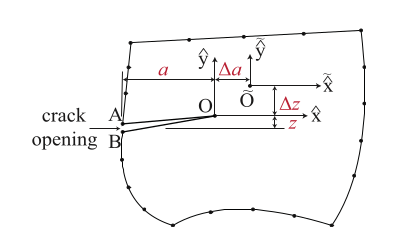
\includegraphics[width=.5\textwidth]{s17.png}}
    \captionsetup{labelformat=empty}
    \caption{Perturbation in scaled boundary coordinates.}  
\end{figure}

\subsection{Fracture Failure Criteria}
\subsubsection{Mode-I failure}
During fracture, the material can be associated with its own characteristic resistance to fracture known as the ’fracture
toughness’ $K_{Ic} $such that the crack will grow under Mode-I loading when
\begin{align*}
    K_I > K_{Ic}
\end{align*}
\subsubsection{Mixed-Mode Failure}
The failure criteria can be simplified, for 2D Mixed-Mode loading, as
\begin{align*}
    &K_{eff} > K_{Ic}\\~\\
    &\text{where,}\\
    &K_{eff} = \cos\frac{\theta_c}{2}\left(K_1 \cos^2\frac{\theta_c}{2}- \frac{3}{2}K_{II}\sin\theta_c\right)
\end{align*}
\subsection{Monte Carlo Simulation (MCS) method}
\subsubsection{The deterministic fracture mechanics problem}
Assume a high toughness material with crack
growth relation, in the range of $\Delta K$ values of interest,
given by
\begin{align*}
    da/dN_{pr} = C\Delta K ^ n
\end{align*}
where $C,\ n$ are empirically determined constants, a is
the radius of a circular crack in the fracture plane,
$\Delta K$ is the range of stress intensity factor, and $N_{pr}$ is
the number of fatigue cycles.
For the case of a buried circular crack remote from
the surface and extending through the uniform tensile
stress field, we have
\begin{align*}
    \Delta K = 2 \Delta \sigma (a / \pi)^{1/2}
\end{align*}
where $\Delta \sigma$ is the range of stress
If these equations are combined and integrated,
the following expression for fatigue life $N_{pr}$ is obtained:
\begin{align*}
    N_{pr} = \frac{a_{i}^{1 - n/2}-a_{f}^{1 - n/2}}{c \Delta \sigma^n(4/\pi)^{n/2}(n/2 - 1)}
\end{align*}
where $n \neq 2$, $a_i$ is the maximum initial and $a_{f}$ is the
final half-crack size. The $a_f$ term is negligible for the
assumed case of a high toughness material with
\begin{align*}
    a_i \ll a_f
\end{align*}

We may write eq. in terms of the fracture plane
defect area $A_i = \pi a_i^2$. The result is
\begin{align*}
    N_{pr} = \frac{(A_i/\pi)^{1/2 - n/4}}{c \Delta \sigma^n(4/\pi)^{n/2}(n/2 - 1)}
\end{align*}
We now consider a buried elliptical crack of
fracture plane area $A_i = \pi c b$ where $c \leq b$ are the major
and minor semi-axes of the elliptical projection of the
flaw on the fracture plane. The results of a more 
advanced analysis, shows
that eq. is reasonably accurate for the elliptical
crack, with $b/c \ll 40$, as well as the circular crack of
equal area for which eq. is derived.
For the purpose of the PFM analysis below, we
compact the notation and take the logarithm of eq. to obtain
\begin{align*}
    \log N = \log B+ p\log C+ q\log \Delta \sigma + r \log A_i
\end{align*}
\subsubsection{Distributions of the input random variables {$C, \Delta \sigma, A_i$}}
For simplicity, assume that all previously observed
scatter in crack growth rate for given $\Delta K$ can be simulated 
by random variation in $C$ rather than by some
complex joint dependent variation of $C$ and $n$. 
Previous analyses indicate that this assumption is accurate
and produces only minor errors. The relationship
\begin{align*}
    da/dN = 6.76 \times 10^{-11} \Delta K^3.32
\end{align*}
is obtained from
C r - M o - V steel crack growth data and is used
to compute median crack growth rates in in./cyc.
For this steel the mean yield stress is $\bar{\sigma = 85 ksi}$.
The above assumptions can be compacted into the
notation
\begin{align*}
    \log C = \bar{N}(\mu_c, S_c)
\end{align*}
that is, log C is a normal random variable with median
and mean $\mu_c = \log (6.76 X 10^{-11})$ and standard deviation 
$S_c$ .
For the example, we further assume a log-normal
stress variation of
$\log \Delta \sigma =\bar{N}(1.5799, 0.1535),$
which means that Ao has a median value of 38 ksi
with 0.1535 standard deviation on log $\sigma a$ due to
stress gradients, and spindle-to-spindle design and
usage variations. The probabilistic stress distribution
shown is formulated from three assumptions. 
These are (1) log-normality; (2) 95\% of the

spindle material, by volume, will encounter 
$\Delta \sigma <0.80 \bar{\sigma}_y$ = 68 ksi; and (3) 95\% of the material volume
will encounter $\Delta \sigma > .25 \bar{\sigma}_y$ = 21 ksi.
Finally we assume the flaw size distribution that
is used to determine $A_i$ obeys the relation $\log A_i = \bar{N}( -0.9586, 0.750).$
\begin{figure}[H]
    \centering
    \fbox{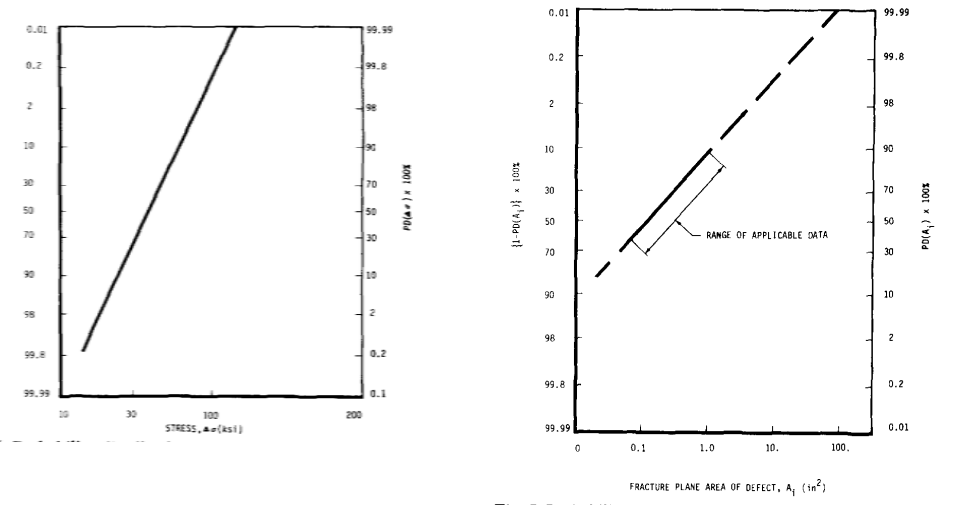
\includegraphics[width=\textwidth]{s23.png}}
    \captionsetup{labelformat=empty}
    \caption{Probability distribution of turbine rotor spindle alternating stress level}  
\end{figure}

\subsubsection{The probabilistic analysis}
We assume that each rotor spindle must endure
the equivalent * of 3000 cycles in service, where each
cycle comprises a cold start-up, operation and shut-
down. The assumption of constant usage allows a
simple definition of Y such as
\begin{align*}
    Y = N_{pr} = N_{pr}(C, \Delta\sigma, A_i)
\end{align*}
and the probability of failure is P(E) = P(Y < 3000
cycles).
To obtain an analytical solution for the distribution of fatigue life, we utilize the following theorem
\begin{align*}
    &X_1 = \bar{N}(\mu_1, S_1),    X_1 = \bar{N}(\mu_1, S_1)\\
    \\&Y = P_1 X_1 + P_2 X_2 + P_3\\
    \\&Y = \bar{N}(\mu_y, S_y)\\
    \\&\mu_y = P_1 \mu_1 + P_2 \mu_2 + P_3\\
    \\&S_y = (P_1^2 S_1^2 + P_2^2 S_2^2)^(1/2)\\
\end{align*}
The numerical results are\\\\
$\mu_N \log B + p \mu_c + q \mu_\sigma + r\mu_A = 5.4113$\\\\
$S_N = (p^2 S_c^2 + q^2 S_\sigma^2 + r^2 S_A^2) = .5763$\\\\
The number of cycles at a given failure probability $\alpha$ is simply\\\\
$N_{pr} = 257800(10^{k \alpha})^{.5763}$\\\\
and $k_\alpha$ is the standard deviate corresponding to particular $\alpha$
\begin{figure}[H]
    \centering
    \fbox{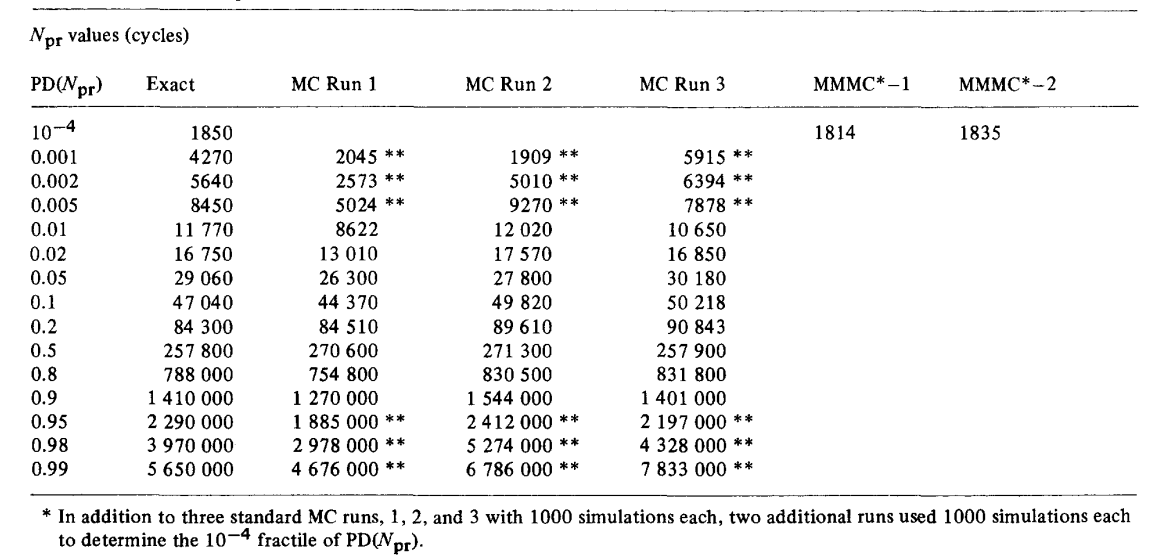
\includegraphics[width=\textwidth]{s24.png}}
    \captionsetup{labelformat=empty}  
\end{figure}
\subsubsection{Shape Sensitivity Analysis}
\begin{figure}[H]
    \centering
    \fbox{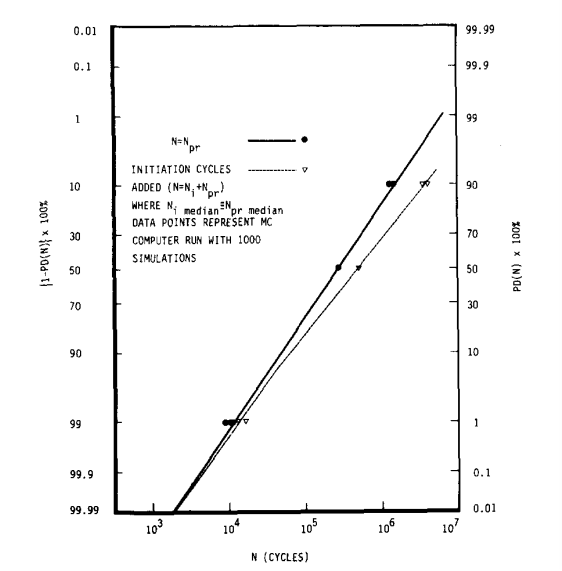
\includegraphics[width=.4\textwidth]{s25.png}}
    \captionsetup{labelformat=empty} 
    \caption{Probability distribution of fatigue lifetime of defected turbine rotor spindle} 
\end{figure}
\subsubsection{Shape Sensitivity Analysis}



\subsubsection{Direct Monte Carlo Reliability}
The Monte Carlo Simulation (MCS) method is widely accepted as a logical tool for modeling structural behavior with significant 
uncertainties or randomness of input parameters. The execution of the method is very simple and versatile for
engineering applications. A $N$-dimensional random vector {\bf X} with components {\bf X} = $(X_1 , X_2 , . . . , X_N )$ characterizing the 
uncertainties in the input parameters such as the load, crack geometry, and material properties is considered. For instance, if
the crack size a, elastic modulus E, the far field applied stress $\sigma^\infty$ , and the Mode-I fracture toughness $K_{Ic}$ are all random input
variables, then \textbf{X} = \textbf{X}$(a, E, \sigma^\infty , K_{Ic} )$ applies. The structure is deemed to fail if the computed SIF K > $K_{Ic}$ . To be precise, Mode-I
failure is dictated by $K_I > K_{Ic}$ while for Mixed-Mode it is ${K_{eff} > K_{Ic} }$, as mentioned earlier. Clearly, this
requirement cannot be satisfied de-terministically as $K$ is dependent on the random vector while $K_{Ic}$ is also random. Note
that, rather than depending on customized response surface approximations, the randomness in crack size $a$ is accounted
for by the response matrix $[K_s ]$ obtained with the SBFEM.

The methodology of the MCS reliability prediction is as follows. The random input variables may or may not be statistically 
independent of each other. Given their specific statistical parameters, each input variable is randomly generated from
some prescribed probability distribution function, based on which the response variable is calculated. This process encompasses 1 MCS 
cycle and the constituents within the cycle are together taken as 1 sample point. Examples of commonly used
distributions for probabilistic analysis include the Gaussian, or normal, distributions defined by


\begin{align*}
    f(x) = \frac{1}{\sqrt{2 \pi S^2}}e^{-\frac{(x - \mu )^2}{2 S^2}}\\~\\
\text{and lognormal distribution is given by}\\~\\
    f(x) = \frac{1}{x\sqrt{2 \pi S^2}}e^{-\frac{(\ln x - \mu )^2}{2 S^2}}\\ \tag{28}
\end{align*}

where $f(x)$ is the probability density function, and $S$ and $\mu$ are statistical parameters. The coefficient of variation $COV$ is expressed as
\begin{align*}
    COV = S/\mu \tag{29}
\end{align*}

A large number of such MCS cycles are performed to collect the equal number of sample points. A statistical analysis is 
carried out for all the sample points to obtain statistical parameters such as the mean $\mu$ , standard deviation $S$, and coefficient of
variation $COV$ of the response variable (i.e. SIFs \{$K$\}). Likewise, for each sample an analysis is carried out to evaluate failure,
i.e. $K > K_{Ic}$ . Letting $N_F$ be the number of simulations when $K$ exceeds $K_{Ic}$ and $N$ to be the total number of simulation cycles, the
estimation for the probability that failure has occurred, $P_F$ , can be directly expressed by

\begin{align*}
    P_F = \frac{N_F}{N} \tag{30}
\end{align*}
Inevitably, the MCS method would require a sufficient number of entries in the response matrix [K s ] for a reliable 
probabilistic analysis, particularly when the uncertainty in crack size is very high.

\subsubsection{First-Order Second-Moment (FOSM) Reliability}
Although it can be determined computationally, the probability of failure P F is also commonly represented by the integral
\begin{align*}
    P_F = \int_{g(\text{X}) \le 0} f_{\text{X}}(\text{X})d\text{X} \tag{31}
\end{align*}
where X is the vector of random variables, $f_\text{X}$ (X) is the joint probability density function, and g(X) is the performance function
which is given by
\begin{align*}
    g(X) = K_{Ic} - K
\end{align*}
The integral is difficult to evaluate explicitly due to multiple integrals that need to be performed, while the joint
probability density function itself is complicated to attain statistically. Often, a first-order approximation technique of the
integral is required. A simple example of this is the first-order second-moment (FOSM) method. The controlling 
characteristic parameter of the FOSM is defined as the Cornell reliability index $\beta$
\begin{align*}
    \beta = \frac{\mu_{K_{Ic}}-\mu_K}{\sqrt{S_{K_{Ic}}^2 - S_K^2}} \tag{32}
\end{align*}

where $\mu$ and $S$ , are the statistical mean values and the standard deviations of the fracture toughness $K_{Ic}$ and
stress intensity factor (SIF).Using this index, the probability of failure is approximated by
\begin{align*}
    P_F = \phi(-\beta) \tag{33}
\end{align*}
where $\phi(u)$ is the cumulative probability distribution function and is given by
\begin{align*}
    \phi(u) = \frac{1}{\sqrt{2 \pi}}\int_{-\infty}^{u} e^{\frac{-t^2}{2}}  \tag{34}
\end{align*}
\subsection{Summary Of Monte Carlo Probabilistic Method}
The reliability of cracked structures are evaluated by a Monte Carlo probabilistic method. Uncertainties in the crack configuration 
are modeled using a shape sensitivity approach with the aid of the scaled boundary finite element method
(SBFEM). In contrast to the finite element method, efficiency, simplicity, and versatility in achieving this task is recognizable
with the SBFEM since no fine internal meshing nor remeshing is necessary for shape sensitivity calculations, noticeably
reducing computational effort. Comparative studies show good agreement with results obtained from references. For the
same problem, considerably lesser number elements and nodes are required. Indeed, the SBFEM can substantiate for 
accurate probabilistic fracture analysis. The present technique can also be extended to study the reliability of structures with
multi-cracks


\rule{\textwidth}{.1em}
\subsection{Edge-Cracked Plate Under Uniaxial Tension (Mode-I) With Varying Crack Length(Example)}
The edge-cracked rectangular plate has dimensions 2L and W. The upper and lower ends of the plate are subjected
to tensile stress r 1 . The crack is horizontal and its length a varies. This is an example of a Mode-I problem.

\begin{figure}[H]
    \centering
    \fbox{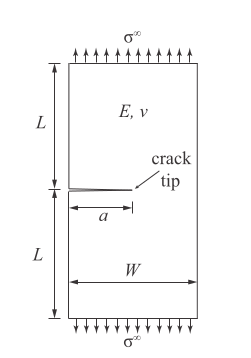
\includegraphics[width=.3\textwidth]{s18.png}}
    \captionsetup{labelformat=empty}
    \caption{Horizontal edge-cracked plate under uniaxial tension}  
\end{figure}
\subsubsection{Shape Sensitivity Analysis}
Coinciding with $g(X) = K_{Ic} - K$, the dimensions of the plate is chosen as $L/W = 1$ with far-field applied tensile stress $\sigma^\infty$ = 1 unit. The
elastic material properties are taken as Young’s modulus$ E = 20.7 x 10^6 $units and Poisson’s ratio$\nu$ = 0.3. The normalized
crack length $a/W$ is varied from 0.1-0.8. For relatively small crack sizes $a/W \le 0.2$ the rectangular plate is divided into 3
sub-domains (Fig. a) with 14 elements (210 nodes), while for larger crack sizes $0.2 < a/W \le 0.8$ only 1 sub-domain is used
(Fig. b) with 12 elements (190 nodes).

\begin{figure}[H]
    \centering
    \fbox{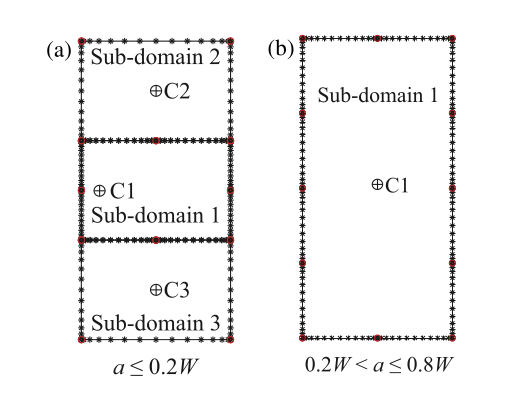
\includegraphics[width=.6\textwidth]{s19.png}}
    \captionsetup{labelformat=empty}
    \caption{Mesh of horizontal edge-cracked plate: (a) 3 sub-domain mesh; (b) 1 sub-domain mesh.}  
\end{figure}
The computed normalized Mode-I stress intensity factor (SIF) $K_1/\sigma\sqrt{\pi a}$ is plotted as a variation of the normalized crack
length $a/W$ . Note that this is reflective of the Mode-I response matrix [$K_s$ ]. Acceptable convergence is achieved using
9-node, 11-node, and 15-node elements . The corresponding derivative $\partial K_I/\partial a$ is calculated and plotted. 
Analytical solutions are also provided for an infinite domain (i.e. $L/
W = \infty$).
\begin{figure}[H]
    \centering
    \fbox{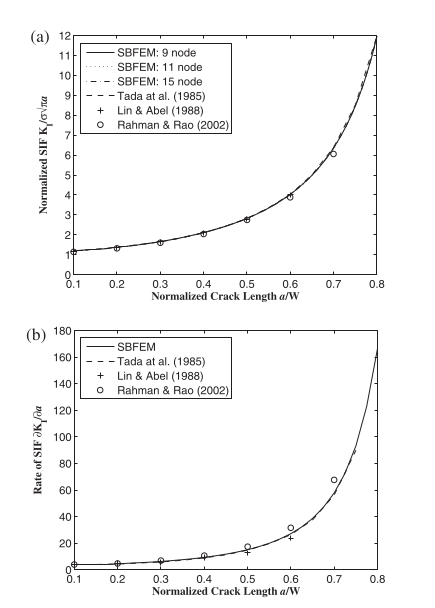
\includegraphics[width=.7\textwidth]{s20.png}}
    \captionsetup{labelformat=empty}
    \caption{Horizontal edge-cracked plate under uniaxial tension: (a) normalized Mode-I (b) rate of Mode-I}  
\end{figure}
{\it Probabilistic analysis } A probabilistic analysis is carried out for the same plate. Adopting the dimensions of the plate
are taken to be W = 0.508 m  and 2L = 5.08 m  (i.e.$L/W = 5$) with randomness (uncertainty) in the applied farfield
 tensile stress of r 1 , crack length a, Young’s modulus $E$ and Poisson’s ratio $\nu$ , and fracture toughness $J_{Ic}$ . The Mode-I response 
 matrix [$K_s $] is calculated using the scaled boundary finite element method (SBFEM). For the sake of comparison with
the aforementioned reference, the value of the J-integral, yet another fracture parameter commonly used in probabilistic
analysis, is determined by the Griffith-Irwin relation given as $J = K^2 /E$ for the plane stress condition. The load, crack size,
and material properties are treated as statistically independent random variables. The Monte Carlo simulation (MCS)
method is used to determine the probability of failure P F . The mean far-field tensile stress is indicated as $E[\sigma^\infty$] where E[.] is
the expectation (mean) operator. Figure plots the probability of failure P F VS . the mean far-field tensile stress $E[\sigma^\infty$] for both
the deterministic ($COV^{a/W}$ = 0\%) and random ($COV^{a/W}$ = 5\%, 10\%, and 15\%) crack sizes. As expected, the results indicate that the
failure probability increases with the $COV^{a/W}$(uncertainty).The failure probability can be much larger than the probabilities
calculated for a deterministic crack size, particularly when the uncertainty of a/W is large.
\begin{figure}[H]
    \centering
        \fbox{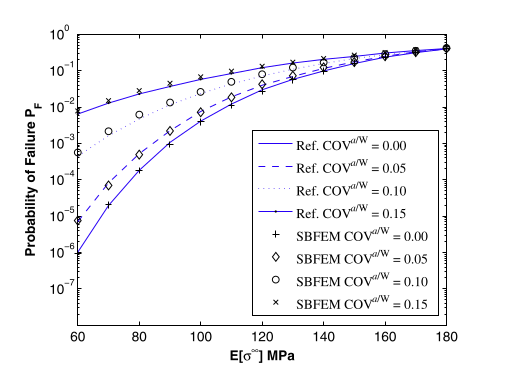
\includegraphics[width=.5\textwidth]{s21.png}}
    \captionsetup{labelformat=empty}
    \caption{Failure probability of horizontal edge-cracked plate under uniaxial tension for varying uncertainty}  
\end{figure}


\rule{\textwidth}{.1em}
\section{Conclusion}
$\Rightarrow$ Fracture initiation and stable crack growth are local fracture phenomena. Therefore, in order to
apply the energy principle, the variation of the local crack tip stresses and strains and the associated
detailed fracture process have to be taken into consideration
\\\\$\Rightarrow$ Fracture toughness is the measure of the fracture ductility of a material. The fracture ductility of
a material is a function of the superimposed hydrostatic tensile stress. The tearing modulus is the
measure of the increase in fracture ductility as the hydrostatic tension is reduced when the fr icture
surface changes from mode I to a combination of modes I, II, and III during stable crack growth.
\\\\$\Rightarrow$ In order to extend fracture mechanics beyond the realms of K and J, the fracture mechanism has
to be found, the crack tip stress and/or strain directly responsible for the fracture process has to be
established, and the local stresses and strains have to be related to far field parameters.
\\\\$\Rightarrow$ The stress smoothing error estimators highlighted in this work seem to offer many advantages.
They appear to be robust and efficient. Further work is needed in comparing these and other
estimators so that they can be incorporated into a commercial adaptive FE program.
There are many other areas of the adaptive FEM that need to be investigated, such as error
estimators, solution algorithms, extension to three dimensions, non-linear and dynamic analyses
and the incorporation of these in an optimized user-friendly environment using ideas of
knowledge-based systems and expert systems for fracture-proof design
\\\\$\Rightarrow$ A probabilistic fracture mechanics (PFM) anal-
ysis is often necessary in order to achieve accurate
estimates of reliability of structural components and
to study the effects on reliability of systematic and
stochastic variation in controlling parameters.
\\\\$\Rightarrow$To enhance future PFM applications, data col-
lection efforts should seek to quantify the variational
characteristics and the uncertainties of the studied
parameters. In this manner, a data base of input pa-
rameter probability distributions can be formed to
facilitate future PFM and other engineering probabili-
ty and risk analyses.
\\\\$\Rightarrow$ The reliability of cracked structures are evaluated by a Monte Carlo probabilistic method. Uncertainties in the crack con-
figuration are modeled using a shape sensitivity approach with the aid of the scaled boundary finite element method
(SBFEM). In contrast to the finite element method, efficiency, simplicity, and versatility in achieving this task is recognizable
with the SBFEM since no fine internal meshing nor remeshing is necessary for shape sensitivity calculations, noticeably
reducing computational effort. Comparative studies show good agreement with results obtained from references. For the
same problem, considerably lesser number elements and nodes are required. Indeed, the SBFEM can substantiate for accu-
rate probabilistic fracture analysis. The present technique can also be extended to study the reliability of structures with
multi-cracks.





\end{document}  
